\documentclass{beamer}

\usepackage{xcolor}

% Symbols etc.
\usepackage{amsmath}
\usepackage{amssymb}
\usepackage{siunitx}   % Units
\usepackage{physics}   % Highly controversial package... can comment out 
\usepackage{upgreek}   % Upright greek letters
\usepackage{cancel}    % Cancel (slash) terms in an equation
\usepackage{slashed}   % Feynman slash
\usepackage{tikz}

\usepackage{subcaption} % Subfigures

\usetikzlibrary{arrows,shapes}
\usetikzlibrary{backgrounds}
\usepackage{annotate-equations}
% \usefonttheme{professionalfonts}
\usefonttheme[stillsansseriflarge,stillsansserifsmall]{serif}
% Change annotate-equation text
\newcommand{\eqnannotationtext}[1]{\sffamily\normalsize#1\strut}

% Theme choice:
\usetheme{Antibes}

% Colors
\input{/Users/lzawbrito/latex-templates/color-palette.tex}

\setbeamercolor{palette primary}{bg=myblue}
\setbeamercolor{palette secondary}{bg=myblue!70!black}
\setbeamercolor{palette tertiary}{bg=myblue!60!black}
\setbeamercolor{palette quaternary}{bg=myblue!50!black}

\setbeamercolor{item}{fg=black}
\setbeamercolor{block title}{bg=myblue!80!black}
\setbeamercolor{block title alerted}{bg=myred!80!black}
\setbeamercolor{block title example}{bg=mygreen!80!black}

% Title page details: 
\title{Physics, Backwards: Hamiltonian Reconstruction} 
\author{Lucas Z. Brito}
\date{\today}
\logo{\large \LaTeX{}}
\institute{Brown Physics DUG Scialogue}

% Customizations
\setbeamertemplate{navigation symbols}{} % Remove nav buttons
\useoutertheme[footline=empty,subsection=false]{miniframes}
\useinnertheme{circles}

\begin{document}
% Title page frame
\begin{frame}[plain]
    \titlepage 
\end{frame}

\section{Introduction}
\begin{frame}{Collaborators}
\begin{figure}[t]
\captionsetup[subfigure]{labelformat=empty}
\centering
\begin{subfigure}{0.33\textwidth}
	\centering
	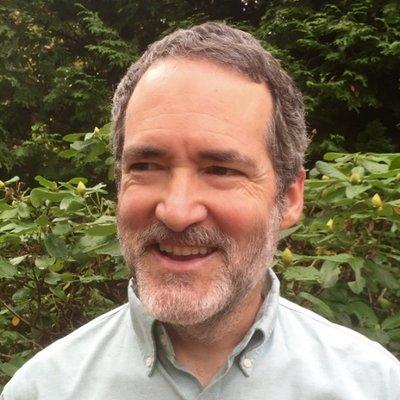
\includegraphics[width=75pt]{figs/marston.jpg}
	\caption{Brad Marston}
\end{subfigure}%
\begin{subfigure}{0.33\textwidth}
	\centering
	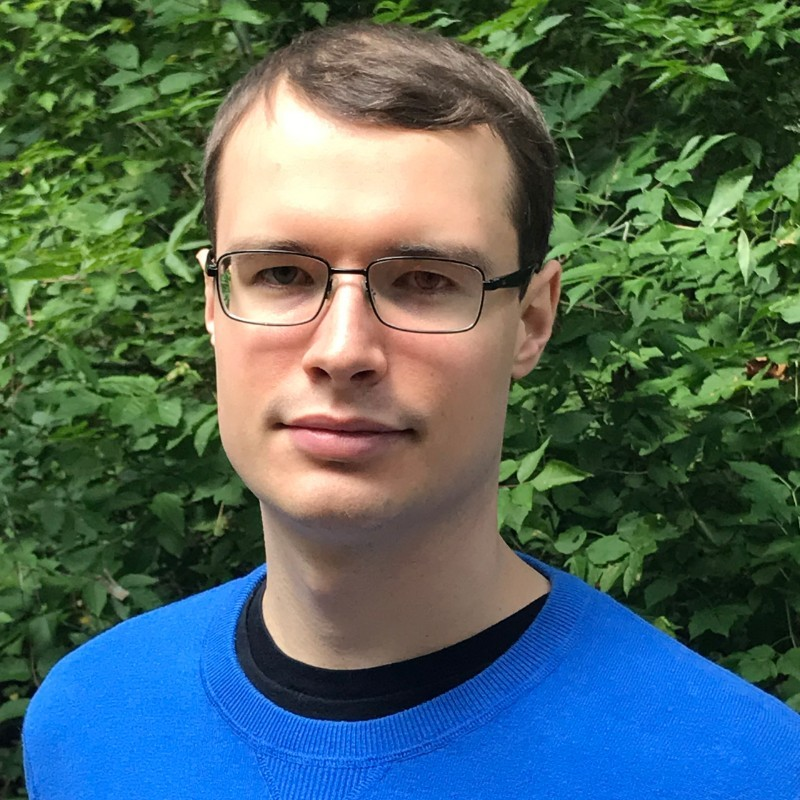
\includegraphics[width=75pt]{figs/carr.jpg}
	\caption{Stephen Carr}
\end{subfigure}%
\begin{subfigure}{0.33\textwidth}
	\centering
	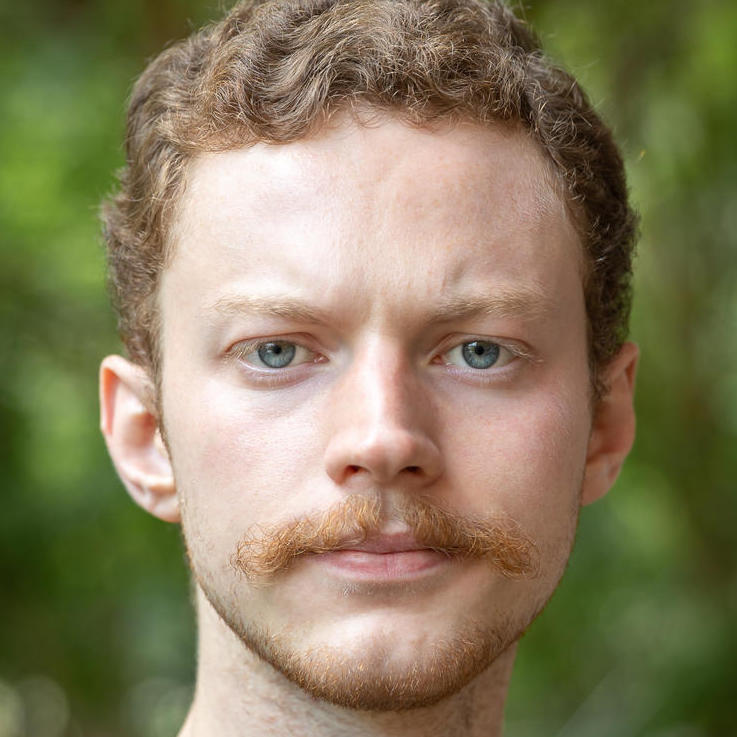
\includegraphics[width=75pt]{figs/jacoby.jpg}
	\caption{Alex Jacoby (Princeton)}
\end{subfigure}
\end{figure}
\begin{figure}[h]
	\centering
	
\includegraphics[width=0.4\textwidth]{figs/princeton-brown.png}
\end{figure}
\end{frame}

\begin{frame}{Preliminaries}
\begin{itemize}
\item<+-> Project in quantum many-body physics, condensed matter theory
\item<+-> QM: Hamiltonian $ H $ determines physics of the system 
\item<+-> System corresponding to $ H $ can be found in a state 
\begin{equation*}
	\ket{\psi} \text{ eigenvector of } H 
\end{equation*}
\item<+-> $ H $ function of operators (observable quantities)
\end{itemize}
\begin{block}{Physics, Backwards}<+->
	\vspace{-1em}
	\begin{align*}
		&\textbf{Usually:}&& H \longrightarrow \ket{\psi}\\
		\onslide<+->{&\textbf{Hamiltonian reconstruction:}&& \ket{\psi} \longrightarrow H}
	\end{align*}
\end{block}
\end{frame}

\begin{frame}{Quantum Many Body Systems}
\begin{columns}
\begin{column}{0.5\textwidth}
\begin{itemize}
\item<+-> Ignore translational freedom (lattice) 
\item<+-> Focus on spin of particles 
\item<+-> Write Hamiltonian in terms operators $ O_i $ on each 
	point in the lattice
\item<+-> Model of interest: Haldane-Shastry model
\end{itemize}
\end{column}
\begin{column}{0.5\textwidth} %% 
\begin{center}
	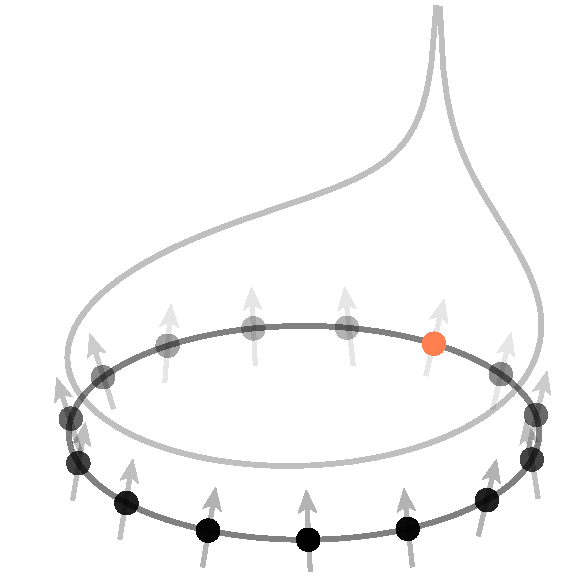
\includegraphics[width=1\textwidth]{figs/hs-hamiltonian-cropped-arrows.pdf}
\end{center}
\end{column}
\end{columns}
\end{frame}

\section{The Correlation Matrix}
\begin{frame}{The Correlation Matrix}
	\begin{exampleblock}{Big Picture}<+->
		\begin{center}
			The entanglement of a state characterizes the 
			Hamiltonian that state solves 
		\end{center}
	\end{exampleblock}
	\begin{itemize}
	\item<+-> Due to Qi and Ranard (2019)
	\item<+-> Fix some state $ \ket{\psi} $, $ \bra{\psi}O_i\ket{\psi} = \langle O_i \rangle$
	\item<+-> Correlation matrix: 
	\begin{equation*}
		M_{ij} = \langle O_i O_j \rangle_\psi - \langle O_i \rangle_\psi 
			\langle O_j \rangle_\psi
	\end{equation*}
	\end{itemize}
\end{frame}

\begin{frame}{Reconstructing with the CM}
\begin{itemize}
	\item<+-> Hamiltonian $ H = \sum_i h_i O_i $
	\begin{equation*}
	\langle H^2 \rangle_\psi - \langle H \rangle^2_\psi = 0
	\end{equation*}
	\item<+-> Diagonalize $ M_{ij} $: 
	\begin{equation*}
		\text{M}
		= 
		\begin{bmatrix}
		{\color{myred}\vb{h}^T}\\  \vb{v}_1^T \\ \vdots  \\\vb{v}_{n-1}^T \\\vb{v}_n^T
		\end{bmatrix}
		\begin{bmatrix}
		{\color{myred} 0} & & & & \\
		& \lambda_1 & & & \\
		& & \ddots & & \\ 
		& & & \lambda_{n-1} & \\
		& & & & \lambda{n} 
		\end{bmatrix}
		\begin{bmatrix}
		{\color{myred}\vb{h}}&  \vb{v}_1 & \cdots & \vb{v}_n
		\end{bmatrix}
	\end{equation*}
\end{itemize}
\begin{block}{}<+->
	\begin{itemize}
		\item $ \vb{h} = [h_1, \dots, h_n] $ are the coefficients of $ H = \sum_i h_i O_i $!
		\item The Hamiltonian is in the nullspace of $ M_{ij} $
	\end{itemize}
\end{block}
\end{frame}

\begin{frame}{Our Work}
\begin{alertblock}{Caveat}<+->
\begin{center}
\LARGE
How do we pick $ O_i $?
\end{center}
\end{alertblock}
\onslide<+->{Our approach:}
\begin{itemize}
\item<+-> Start with a known Hamiltonian, deliberately choose incorrect $ O_i $
\item<+-> See if you can diagnose $ O_i $ from error
\item<+-> (My task) validate with the Haldane-Shastry model
\end{itemize}
\end{frame}

\section{Interlude}
\begin{frame}{Interlude: The Research Workflow}
	\begin{columns}
	\begin{column}{0.6\textwidth}
	\begin{itemize}
	\item<+-> Pen-and-paper calculations and numerical work 
		\begin{itemize}
		\item<+-> Quantum mechanics, SU(2) algebra calculations, second quantization
		\item<+-> Computations with Julia 
		\item<+-> $ 2^{21} \times 2^{21} = 2\, 097\, 152 \times 2\, 097\, 152 $
		matrix!
		\end{itemize}
	\item<+-> Making figures/visualizations to understand numerics
	\item<+-> Going back to analytical calculations to understand results
	\end{itemize}
\end{column}
\begin{column}{0.4\textwidth} %% 
\begin{center}
	\begin{figure}[h]
		\captionsetup{labelformat=empty}
		\centering
		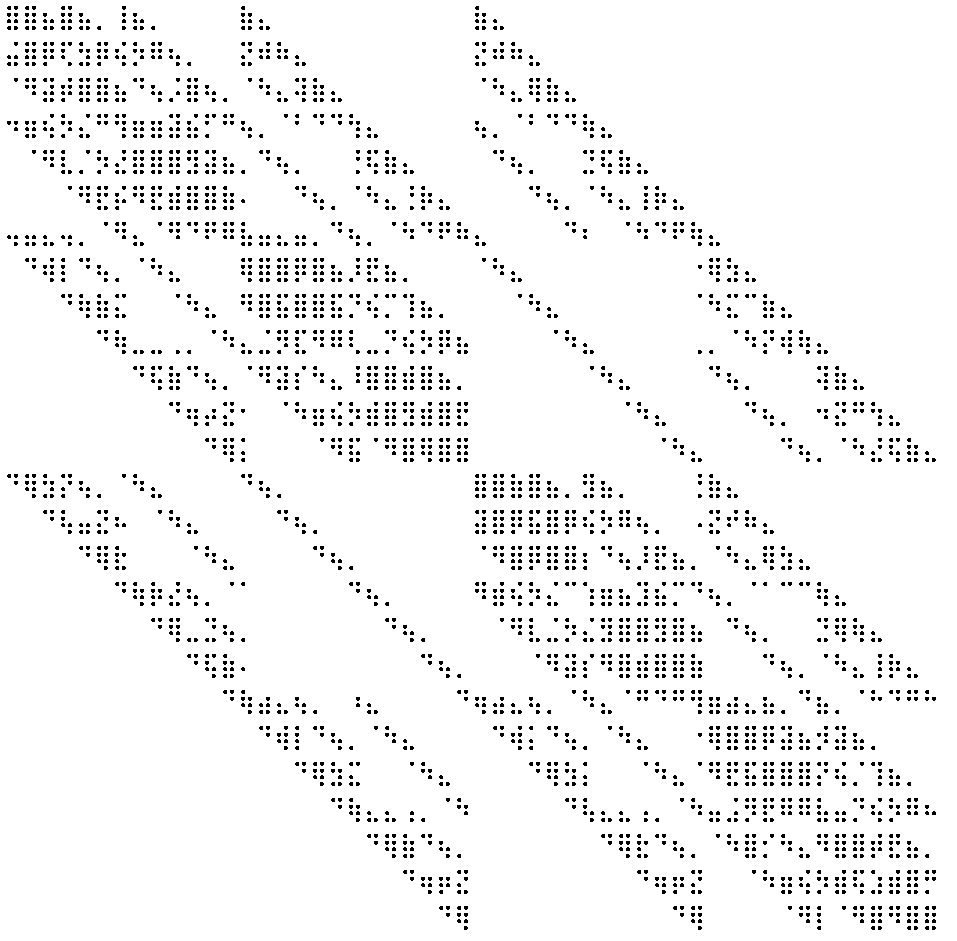
\includegraphics[width=1\textwidth]{figs/matrix_example_inverted.png}
		\caption{\footnotesize Visualization of matrix}
	\end{figure}
\end{center}
\end{column}
\end{columns}
\end{frame}

\section{Diagnosing Failure}
\begin{frame}{Over and Undercomplete Bases}
\begin{exampleblock}{Three Scenarios}<+->
	\begin{itemize}
	\item<+-> \textbf{Case 1:} You have the right amount of operators 
	\item<+-> \textbf{Case 2:} You have too \underline{many} operators (\textit{overcomplete})
	\item<+-> \textbf{Case 3:} You have too \underline{few} operators (\textit{undercomplete})
	\end{itemize} 
\end{exampleblock}
\onslide<+->{What we found: }
\begin{itemize}
\item<+-> \textbf{Case 1:} Everything is (mostly) fine
\item<+-> \textbf{Case 2:} Things might be messed up 
\item<+-> \textbf{Case 3:} Things are messed up, but to a predictable
	degree
\end{itemize}
\end{frame}

\begin{frame}{Over and Undercomplete Bases}
\begin{center}
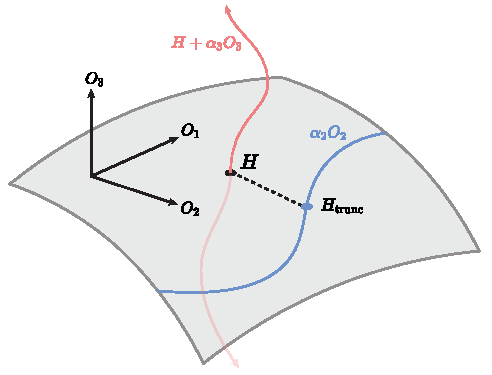
\includegraphics[width=0.8\textwidth]{figs/hrecon_main.pdf}
\end{center}
\end{frame}

\begin{frame}{Case 1: Complete Basis}
\begin{itemize}
\item<+-> Reconstruction should work... \onslide<+->{unless there's a conserved quantity  
$ J = \sum_i j_i O_i$ 
\begin{equation*}
	\qty[ H,J ] = 0 \Longrightarrow  
	\langle J^2 \rangle_\psi - \langle J \rangle^2_\psi = 0
\end{equation*}}
\item<+-> $ J $ leads to extra zero in diagonalization 
\item<+-> Higher dimensional nullspace, diagonalization outputs some 
random vector in that nullspace
\item<+-> Random vector is generally \textit{not} $ \vb{h} $!
\item<+-> E.g., HS has total spin as conserved quantity 
\end{itemize}
\end{frame}

\begin{frame}{Case 2: Overcomplete Basis}
\begin{itemize}
\item<+-> Can think of as having a complete basis then adding new operators
\item<+-> New operator $ O_{i+1} $ might be \textit{irrelevant}
	\begin{itemize}
	\item<+-> Just adds some constant to the energy
	\item<+-> Doesn't affect reconstruction
	\end{itemize}
\item<+-> \textbf{Or...} $ O_{i+1} $ could correspond to a symmetry of $ H $
\item<+-> $ \ket{\psi} $ still solution if you permute operators 
\item<+-> New zero shows up, as in the conserved quantity case above
\end{itemize}
\end{frame}

\begin{frame}{Case 3: Undercomplete}
\begin{columns}
\begin{column}{0.5\textwidth}
\begin{itemize}
	\item<+-> Can think of starting with complete basis and ``truncating'' 
		operators one by one
	\item<+-> Zero eigenvalue $ \lambda_0 $ (in complete basis) deviates from zero
	\item<+-> $\lambda_0 \propto $ magnitude of largest truncated operator in Hamiltonian 
	\begin{equation*}
		H = \sum h_i O_i
	\end{equation*}
\end{itemize}
\end{column}
\begin{column}{0.5\textwidth}
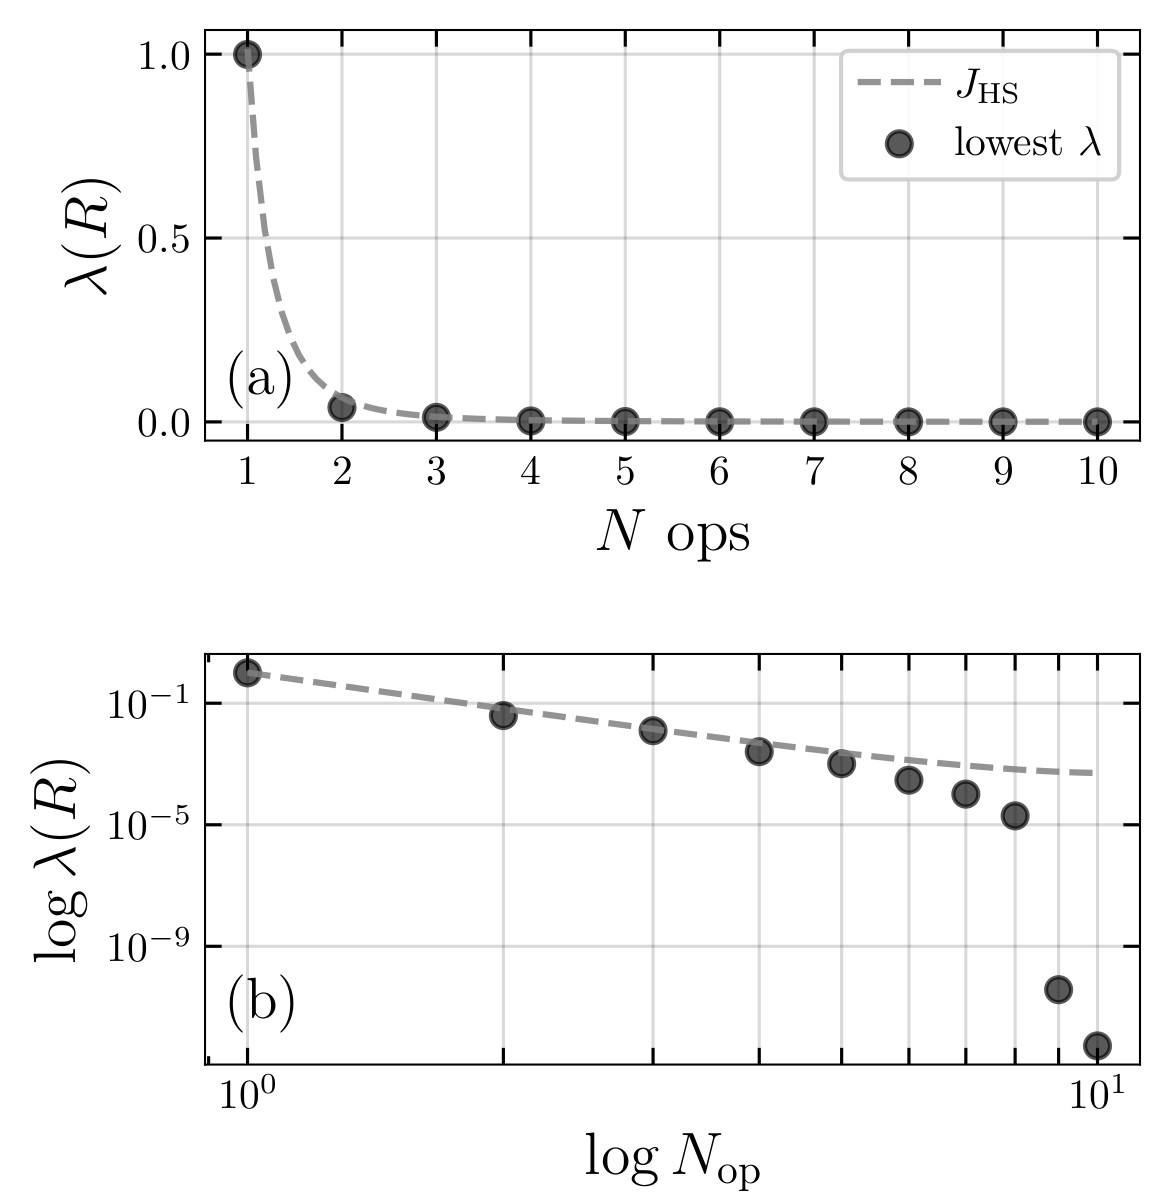
\includegraphics[width=\textwidth]{figs/hs-recon.jpg}
\end{column}
\end{columns}
\end{frame}

\begin{frame}{Next Steps}
	\begin{columns}
	\begin{column}{0.4\textwidth}
		\begin{itemize}
		\item<+-> Currently finalizing figures, paper 
		\item<+-> How to separate conserved quantity from Hamiltonian? 
		\item<+-> Finite-temperature simulations?
		\end{itemize}
	\end{column}
	\begin{column}{0.6\textwidth}
		\begin{figure}[h]
			\centering
			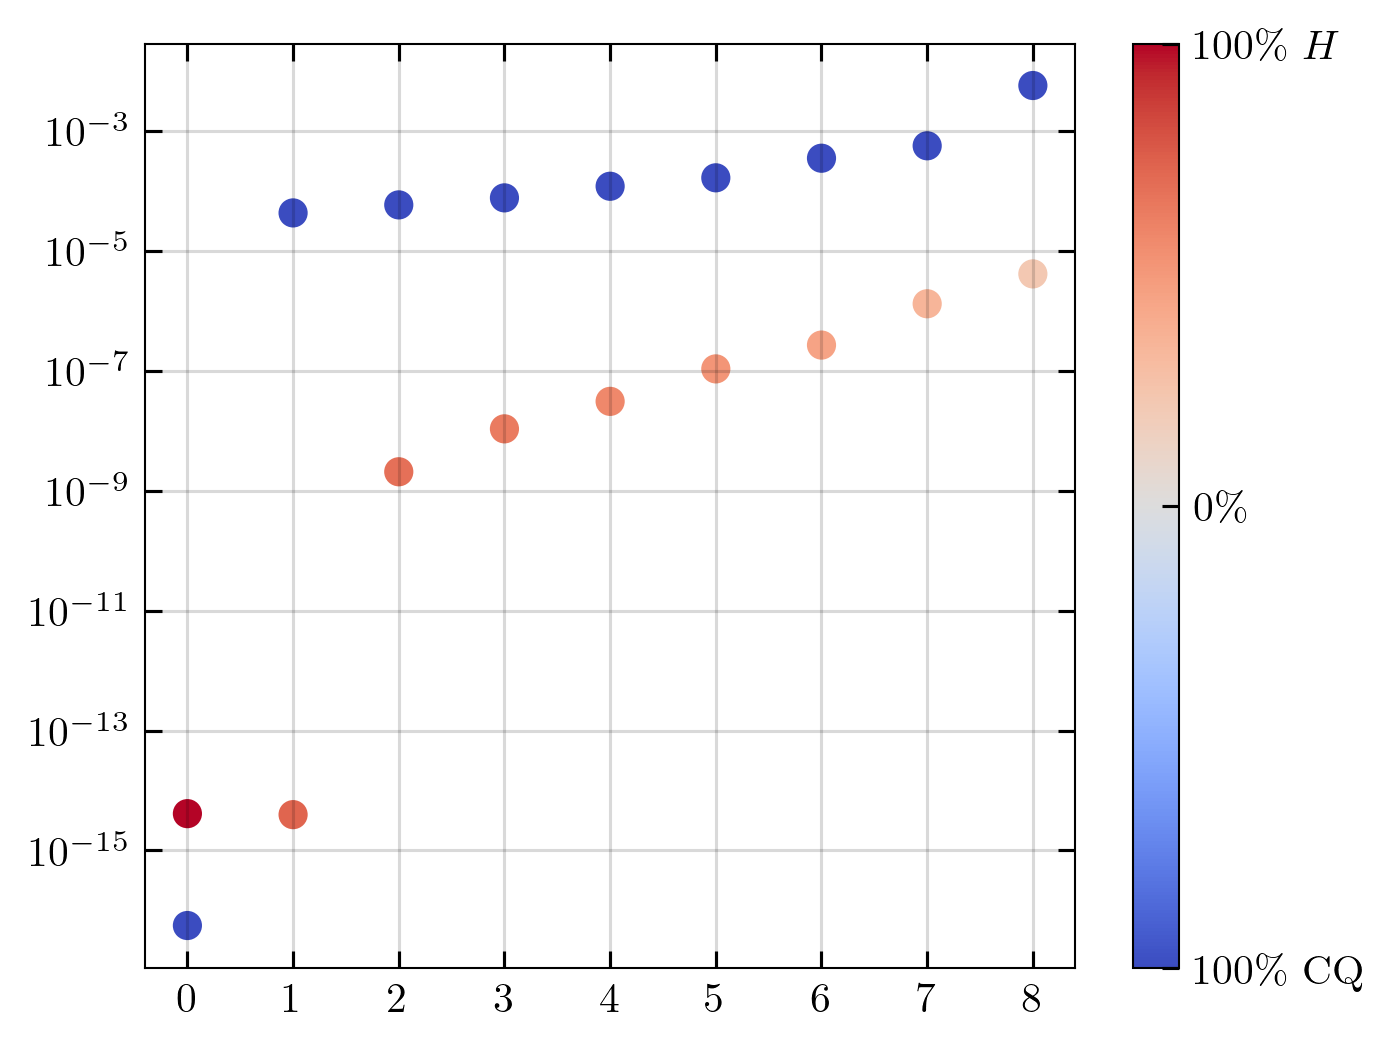
\includegraphics[width=1\textwidth]{figs/cons_quantity_vs_h.png}
		\end{figure}
	\end{column}
	\end{columns}
\end{frame}

\begin{frame}{The End}
\begin{center}
\LARGE Thank you! Questions?
\end{center}
\end{frame}

\end{document}